\gdef\problemNumber{Not in a book}
\def\problemText{
Given the following graph, use Kruskal's algorithm to construct a minimum-cost
spanning tree. Indicate which edges are included and the order in which they are
added.\parend
When sorting, break ties based on the order in which the edges appear in the
LaTeX source code.
\\[12pt]
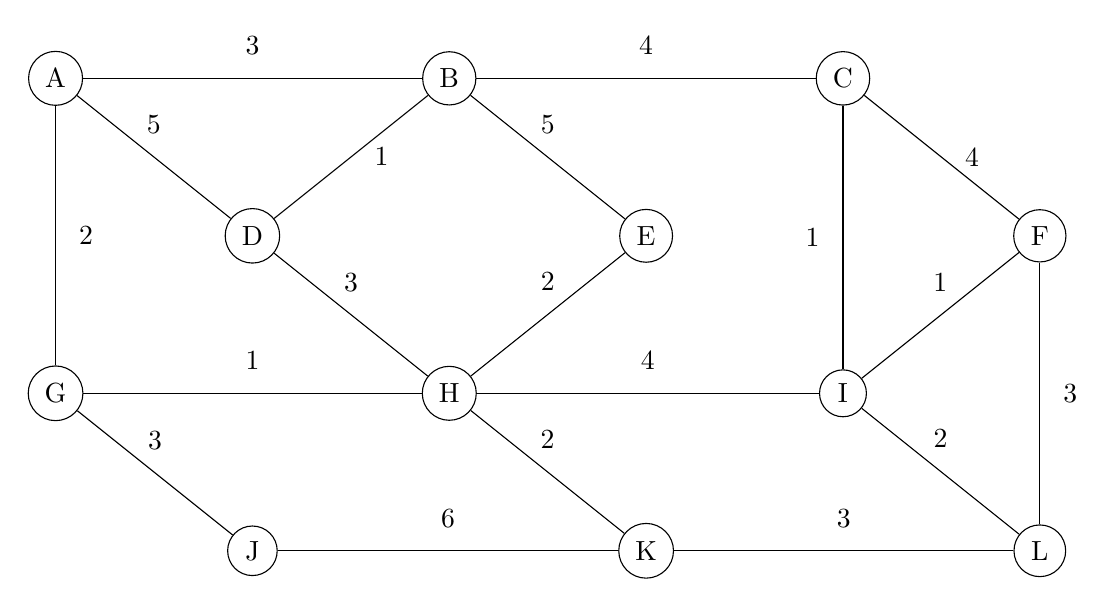
\begin{tikzpicture}
  \node[circle,draw] (va) at (0,6) {A};
  \node[circle,draw] (vb) at (5,6) {B};
  \node[circle,draw] (vc) at (10,6) {C};
  \node[circle,draw] (vd) at (2.5,4) {D};
  \node[circle,draw] (ve) at (7.5,4) {E};
  \node[circle,draw] (vf) at (12.5,4) {F};
  \node[circle,draw] (vg) at (0,2) {G};
  \node[circle,draw] (vh) at (5,2) {H};
  \node[circle,draw] (vi) at (10,2) {I};
  \node[circle,draw] (vj) at (2.5,0) {J};
  \node[circle,draw] (vk) at (7.5,0) {K};
  \node[circle,draw] (vl) at (12.5,0) {L};

  \draw (va) edge node[above=5pt] {3} (vb);
  \draw (va) edge node[above=5pt] {5} (vd);
  \draw (va) edge node[right=5pt] {2} (vg);
  \draw (vb) edge node[above=5pt] {4} (vc);
  \draw (vb) edge node[right=5pt] {1} (vd);
  \draw (vb) edge node[above=5pt] {5} (ve);
  \draw (vc) edge node[right=5pt] {4} (vf);
  \draw (vc) edge node[left=5pt] {1} (vi);
  \draw (vd) edge node[above=5pt] {3} (vh);
  \draw (ve) edge node[above=5pt] {2} (vh);
  \draw (vf) edge node[above=5pt] {1} (vi);
  \draw (vf) edge node[right=5pt] {3} (vl);
  \draw (vg) edge node[above=5pt] {1} (vh);
  \draw (vg) edge node[above=5pt] {3} (vj);
  \draw (vh) edge node[above=5pt] {4} (vi);
  \draw (vh) edge node[above=5pt] {2} (vk);
  \draw (vi) edge node[above=5pt] {2} (vl);
  \draw (vj) edge node[above=5pt] {6} (vk);
  \draw (vk) edge node[above=5pt] {3} (vl);

\end{tikzpicture}
\vskip12pt
}
\def\problemSolution{
\textcolor{blue}{
\textbf{Answer:}\\
This is what the answer should look like. Note that this is not part of a
correct answer.
\\[6pt]
\begin{tabular}{|c|c|c|}
  \hline
  {\bf Edge} & {\bf Cost} & {\bf Used}\\
  \hline
  \hline
  BC & 1 & Yes\\ \hline
  CE & 1 & Yes\\ \hline
  FI & 1 & Yes\\ \hline
  HJ & 1 & Yes\\ \hline
  DE & 2 & Yes\\ \hline
  AB & 3 & Yes\\ \hline
  AF & 3 & No\\ \hline
\end{tabular}
}
}
\gdef\problemOutcomes{CS 2, CS 6, 5870-2}
